\section{Merkmalsselektion}
\label{merkmalsselektion}

Die in Kapitel~\ref{merkmalsextraktion} ermittelten Formmerkmale auf den Knoten eines Graphen, der aus einer Superpixelrepräsentation generiert wurde, besitzen mit $38$ Dimensionen eine hohe Dimensionalität.
Viele der Formmerkmale bauen dabei aufeinander auf und es ist daher fraglich, inwieweit die gesamte Menge der Merkmale gebraucht werden oder ob eine Untermenge dieser ausreicht.
Eine \emph{\gls{PCA}} auf den Merkmalen kann uns helfen, die reale Dimensionalität der Daten abzuschätzen.
Dafür werden die Merkmale durch eine Linearkombination ihrer Hauptkomponenten beschrieben und können so durch weitaus weniger Dimensionen beschrieben werden.
Abbildung~\ref{fig:pca} zeigt dabei die kumulative Varianz des Merkmalraums, \dhe{} die Abdeckung des Raums, in Abhängigkeit zu der Anzahl an Hauptkomponenten der \gls{PCA}.
\begin{figure}[t]
\centering
  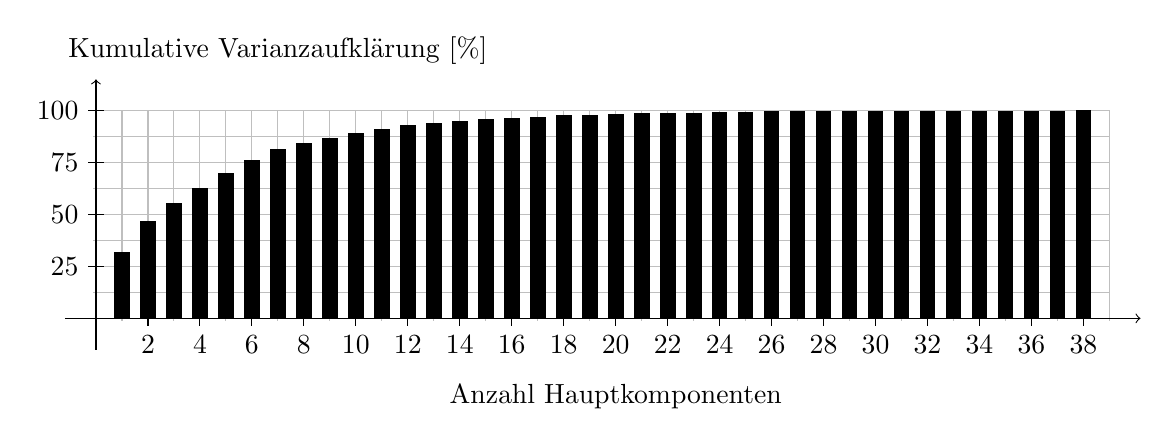
\begin{tikzpicture}[scale=0.33]
  \draw[color=lightgray] (-0.1, -0.1) grid (39, 8);

  \def\values{{
    2.5665,
    3.7289,
    4.4219,
    5.02807,
    5.58180,
    6.11320,
    6.52090,
    6.73047,
    6.93667,
    7.12766,
    7.29462,
    7.43057,
    7.52468,
    7.59263,
    7.65627,
    7.71825,
    7.76556,
    7.80805,
    7.83691,
    7.86244,
    7.88456,
    7.90469,
    7.92110,
    7.93687,
    7.95153,
    7.96374,
    7.97353,
    7.98057,
    7.98486,
    7.98878,
    7.99141,
    7.99388,
    7.99611,
    7.99779,
    7.99861,
    7.99933,
    7.99977,
    8}}

  \foreach \x in {1,2,3,4,5,6,7,8,9,10,11,12,13,14,15,16,17,18,19,20,21,22,23,24,25,26,27,28,29,30,31,32,33,34,35,36,37,38}
    \pgfmathparse{\values[\x - 1]}
    \edef\value{\pgfmathresult}
    \draw[line width=0.2cm] (\x, 0) -- (\x, \value);

  \draw[->] (-1.2, 0) -- (40.2, 0);
  \draw[->] (0, -1.2) -- (0, 9.2);

  \node at (7, 10.3) {Kumulative Varianzaufklärung [\%]};
  \node at (20, -3) {Anzahl Hauptkomponenten};

  \foreach \y in {1,2,3,4}
    \pgfmathtruncatemacro{\label}{25 * \y}
    \draw (0.3, 2*\y) -- (-0.3, 2*\y) node[left] {\label};

  \foreach \x in {1,2,3,4,5,6,7,8,9,10,11,12,13,14,15,16,17,18,19}
    \pgfmathtruncatemacro{\label}{2 * \x}
    \draw (2*\x, 0.3) -- (2*\x, -0.3) node[below] {\label};

\end{tikzpicture}
\caption[Kumulative Varianzabdeckung einer \gls{PCA}]{Kumulative Varianzabdeckung der Hauptkomponenten einer \gls{PCA} \bzgl{} des Merkmalsraums in Abhängigkeit zu der Anzahl an Hauptkomponenten.
Die Merkmale wurden dabei aus den Knotenmerkmalen von $1000$ segmentierten Bildern gewonnen.
Bereits nach wenigen Hauptkomponenten ist der Größteil der erklärten Varianz abgedeckt.}
\label{fig:pca}
\end{figure}

Es zeigt sich, dass nach bereits recht wenigen Komponenten $\left(\approx 9\right)$ der Großteil des Merkmalraums abgedeckt werden kann.
Im Kontext von neuronalen Netzen ist die Verwendung einer \gls{PCA} aber eher untypisch, denn schließlich müssen dafür weiterhin alle $38$ Formmerkmale berechnet werden und daraus schließlich die neuen Merkmale anhand der Hauptkomponenten ermittel werden.
Ein einfacheres Verfahren ist dagegen eine Auswahl an Merkmalen, genannt \emph{Merkmalsselektion}, die die Merkmalsmenge möglichst gut beschreibt.
